%!TEX root = ../proyecto.tex
\chapter{Modelos de Soft Computing considerados.}
\section{Mapas auto-organizados \textit{(Self Organizing Map)}}
A principio de la década de los 80, el científico finlandés Teuvo Kohonen \cite{kohonensom}, planteó un modelo de aprendizaje automático no supervisado y competitivo basándose en el estudio del funcionamiento del córtex cerebral. El modelo planteado, denominado mapa auto-organizado, red auto-organizada o red neuronal de Kohonen, entre otros nombres similares, es una red neuronal artificial, y las principales características que la definen son las siguientes:\\

\begin{itemize}
	\item Es una \textbf{red neuronal artificial}. Esto quiere decir, a grandes rasgos, que la estructura que genera el modelo está basada en una red de múltiples unidades, llamadas ``neuronas'', que se encuentran interconectadas entre sí.
	
	\item La red neuronal de Kohonen tiene \textbf{dos capas}. Una capa de entrada, con tantas neuronas como características o atributos tenga el vector que representa a la muestra que vaya a ser evaluada por la red, es decir, tanto una muestra como la capa de entrada tendrán la misma dimensión y, una característica, podría ser, por ejemplo, la altura o el peso de una persona. La segunda capa es la capa competitiva o capa de Kohonen, de un tamaño a decidir por el usuario y una estructura habitualmente bidimensional, aunque podría perfectamente usarse cualquier otro número de dimensiones.

	\item Asociado a cada neurona de la capa competitiva, tenemos un vector de referencia variable $w_i(t) \in {\rm I\!R}^n, i=1,2, ..., k$, es decir, un vector de ``referencia'' con respecto a la representación vectorial de las muestras estadísticas $\vec{X} = \vec{X}(t) \in {\rm I\!R}^n$ que se corresponden al conjunto de datos de entrada para el entrenamiento del modelo. Estos vectores también son denominados vectores de pesos y, al conjunto de ellos, se le denomina \textit{codebook}. En los casos en los que el algoritmo sea aplicado para realizar clustering, dicho vector representará el valor promedio de los vectores de características de las muestras asociadas al clúster de su neurona. 

	\item Asociado a cada neurona de la capa competitiva, tenemos un vector de pesos sinápticos obtenido a través de las conexiones con la capa de entrada, que es modificado durante el proceso de aprendizaje. A dicho vector de pesos se le llama vector de referencia, y representa el valor promedio de la categoría asociada a esa neurona. El conjunto de todos esos vectores de referencia es denominado \textit{codebook}.

	\item Es un algoritmo \textbf{no supervisado}, es decir, es capaz de encontrar patrones comunes basándose en los datos de la muestra de entrada sin necesidad de que, cuando una muestra entre a la red, se indique a qué categoría pertenece.

	\item Es un modelo \textbf{competitivo}. Cuando se recibe una muestra, todas las neuronas compiten por ser activadas pero sólo la mejor será activada.
\end{itemize}

\begin{figure}
\centering
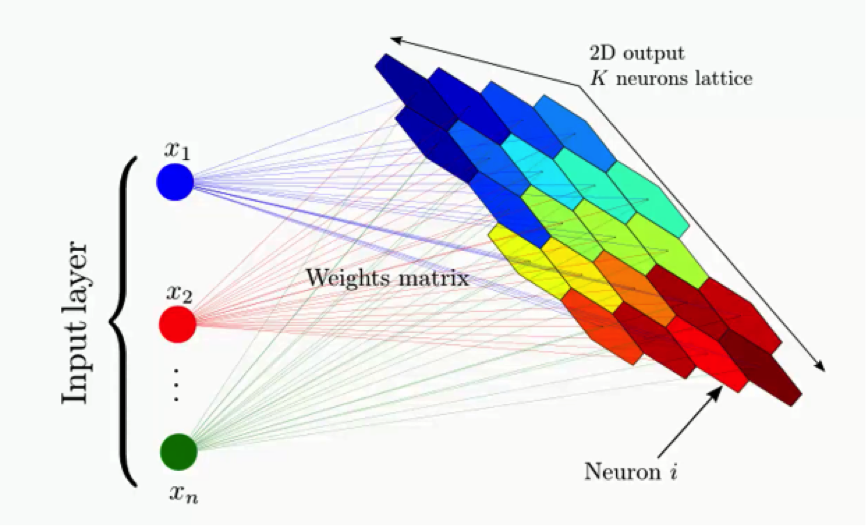
\includegraphics[width=0.8\textwidth]{imagenes/arquitectura_som.png}

\caption{Esquema de una red neuronal de Kohonen.}
%\textit{Autor: Damian Jankowski}
\end{figure}

\subsection{Proceso de entrenamiento.}
\textit{Nota: Por simplicidad en la notación y en la explicación vamos a considerar que la capa competitiva es unidimensional. La explicación propuesta es extensible para un número de dimensiones arbitrario realizando los cálculos relacionados con la posición del vector de referencia dentro del codebook y la posición de la BMU utilizando vectores con un valor para cada una de las dimensiones correspondientes.\\}

Sea $\vec{X}$ un vector, que representa una secuencia de muestras estadísticas de un observable $x=x(t) \in {\rm I\!R}$, donde $t$ es el instante o iteración de la extracción de la muestra y un conjunto de vectores de referencia variables (\textit{codebook}), $w_i(t)$, que representaremos de forma abreviada como el vector $\vec{W(t)}: w_i(t) \in {\rm I\!R} \; | i: 0, 1, 2, ..., n $, donde los $w_i(0)$ están inicializados a un valor aleatorio siguiendo una distribución uniforme entre 0 y 1, se realizan los siguientes pasos, de forma iterativa, hasta alcanzar el número de iteraciones máximo $\lambda$, que determina el usuario como criterio de terminación para el proceso de entrenamiento.\\

En primer lugar, una muestra del vector $\vec{X}$ \textbf{será comparada simultáneamente con cada vector de referencia} $\vec{W(t)} = \{w_0(t), w_1(t), ..., w_i(t), ...,$ ${w_{n-1}}(t)\}$ en cada instante de tiempo $t$, utilizando para ello la distancia euclídea entre vectores, $||{X(t)-w_i(t)}||_n$. Otras formulaciones para la distancia, como por ejemplo, la distancia de Mahalanobis, podrían haber sido usadas en su lugar. \\

A continuación, se determina \textbf{el vector de referencia más parecido a la muestra evaluada} en el instante $t$, y, a la ubicación que ocupa dicho vector de referencia (en índices) en el $codebook$, se le denomina \textbf{BMU \textit{(Best Matching Unit)}}.

$$ BMU(X(t)) = argmin_{w \in \vec{W}}{||X-w||}_n$$

La función $argmin$ devuelve la posición del vector en la que se alcanza el valor mínimo y, a la distancia entre la muestra del instante $t$ y su mejor vector de referencia la denominaremos

$$ D(X(t)) = min_{w \in \vec{W}}{||X-w||}_n$$

Una vez se ha seleccionado la BMU, se inicia un proceso de \textbf{actualización de los vectores de referencia} presentes en el vector $\vec{W}$. La obtención de un mejor ajuste para la siguiente iteración se realiza mediante la actualización del conjunto de vectores de referencia en función de la distancia entre la muestra y la BMU y la posición de la BMU en el vector $\vec{W}$. Este ajuste lo vamos a reflejar añadiendo a cada vector de referencia el término $\Delta W(t)$.

$$\vec{W}(t+1) = \vec{W}(t) + \Delta \vec{W}(t)$$

Durante este fase de actualización, tres parámetros de control pueden ser ajustados por el usuario. El parámetro de control $\tau$ tiene como objetivo marcar el ritmo al que los otros dos, el tamaño del vecindario y la tasa de aprendizaje, decrecen conforme avanza el tiempo siguiendo una función gaussiana. Es habitual utilizar, como $\tau$, el número de iteraciones del proceso de entrenamiento. Por las características de los otros parámetros de control, que vamos a explicar a continuación, un menor valor de $\tau$ permite que el algoritmo realice una transición más rápida de una fase de exploración brusca, en la que gran parte de los vectores de referencia son modificados, a una fase de refinamiento en los que sólo el vector de referencia de la BMU y, quizás, los vectores más próximos, son ligeramente actualizados.\\

El tamaño del vecindario, determina un radio alrededor de la posición de la BMU en el vector $\vec{W(t)}$, en el que los vectores de referencias van a sufrir algún cambio. Si los vectores de referencia no se encuentran dentro del subconjunto $\vec{W_A} = \{w_{BMU(j)-\sigma^2}, ..., w_{BMU(j)}, ..., w_{BMU(j)+ \sigma^2} \}$ su valor para $\delta_i(t)$ será 0. El parámetro $\sigma$ es inicializado en el instante $t=0$ por el usuario y actualizado conforme a una gaussiana. Además del sistema de decrecimiento exponencial presente en la gaussiana, posibilitamos que el usuario determine un valor fijo para $\sigma$, $\sigma_t$ que puede establecerse a partir de una iteración determinada por el mismo, a la que denominamos $z$.


$$\sigma(t) = \left\{
\begin{array}{ll}
\sigma_0e^{-\frac{t}{\tau}} & si \;\;t < z\\
\sigma_f & si  \;\; t\geq z
\end{array}
\right.
$$\\



El tamaño del vecindario, $\sigma$, es utilizado para el cálculo de una función de vecindario, que en función del parámetro $\sigma$ y la distancia (en índices) entre la BMU de cada vector de referencia $\vec{W(t)}$ pondera la modificación que va a ser realizada, permitiendo mantener propiedades topográficas y haciendo que, conforme nos alejamos (en índices) de la posición de la BMU en el vector $\vec{W}$ los cambios realizados sean menores. La función de vecindario, $\delta_f$, viene dada por:

$$\delta_i(t) = e ^{-\frac{||BMU(X(t))-i||}{2\sigma(t)^2}}. $$\\	


En la figura \ref{img:vecindario}, podemos observar una representación gráfica del vector $\vec{W}$ en un codebook bidimensional. Cada uno de los puntos rojos se corresponde con un vector de referencia, la BMU ha sido destacada de color amarillo y la región alrededor de la BMU que va a sufrir cambios significativos, el vecindario, queda delimitada con círculo alrededor de la BMU cuyo radio es $\sigma^2$.
\begin{figure}[H]
\centering
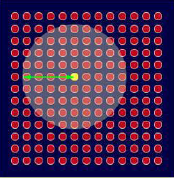
\includegraphics[width=0.3\textwidth]{imagenes/vecindario.png}

\caption{Representación gráfica del vecindario para un codebook bidimensional.}
\label{img:vecindario}
%\textit{Autor: Damian Jankowski}
\end{figure}


Por otro lado, la tasa de aprendizaje, $\eta$, tiene como objetivo ponderar la actualización de los pesos haciendo que, conforme avancen las iteraciones no sólo se vaya reduciendo el número de vectores de referencia que sufren cambios significativos, sino que, además, conforme avance el número de iteraciones incluso el vector de referencia de la BMU reciba cambios más ligeros. De manera similar al tamaño del vecindario, su valor inicial, $\eta_0$ es indicado por el usuario, y se puede establecer una iteración $z$ en la que es fijado a un valor determinado.

$$\eta(t) = \left\{
\begin{array}{ll}
\eta_0e^{-\frac{t}{\tau}} & si \;\;t < z\\
\eta_f & si  \;\; t\geq z
\end{array}
\right.$$\\

Combinando la función de vecindario, la tasa de aprendizaje y la distancia entre la BMU y la muestra a ser evaluada en el instante $t$, obtenemos la fórmula que actualiza los vectores de referencia.

$$\Delta{w_i(t)}=\eta(t)\delta_i(t)(X(t)-w_i(t))$$


Una vez alcanzado el número de iteraciones máximo, el vector $\vec{W}$ contiene los vectores de referencia de la solución de tal manera que si, el algoritmo estuviese siendo usado para resolver problemas de clustering, cada vector de referencia representaría un clúster.

\begin{figure}[H]
\centering
\includegraphics[width=1.0\textwidth]{imagenes/somtraining.png}
\caption{Proceso de entrenamiento de una red neuronal de Kohonen.}
%\textit{\space\space\space\space\space\space\space\space\space Licencia: CC BY-SA 3.0; Autor: Dan Stowell (MCLD)}
\label{img:somtraining}
\end{figure}

La figura \ref{img:somtraining} nos muestra, a grandes rasgos, un esquema del proceso de entrenamiento del mapa auto-organizado de Kohonen con una capa competitiva bidimensional.\\

En la primera parte de la figura, observamos la selección de la BMU. Para ello, del conjunto de datos de entrenamiento (sección azul) se selecciona una muestra de forma aleatoria (círculo blanco) y se toma como mejor neurona del mapa (cada neurona es una intersección de la malla de líneas y, la mejor, es resaltada con un círculo amarillo intenso) la neurona que está más cerca de la muestra.\\

En la segunda parte, observamos el proceso de actualización de los pesos de las neuronas. En este paso, la BMU más cercana se mueve hacia la posición de la muestra, y, las neuronas dentro de su vecindario (círculo amarillo menos intenso), se acercan también a la muestra pero en un menor grado.\\

Por último, vemos cómo, tras un número de iteraciones, el mapa es capaz de ofrecer una aproximación de la distribución de los datos.
\subsection{Usos del mapa auto-organizado.}
El modelo del mapa auto-organizado puede ser utilizado para diversas tareas, de entre las que destacan:\\

\begin{itemize}
	\item \textbf{Clustering} - es decir, generar agrupaciones del conjunto de datos de entrada. Por regla general, cada neurona de la capa de Kohonen representaría una posible agrupación de los datos. 

	\item \textbf{Visualización de datos de alta dimensionalidad.} Tras finalizar el proceso de entrenamiento, podemos utilizar diferentes técnicas para obtener una representación visual de las características topológicas de la muestras. Las matrices-U, las matrices-P o los planos de componentes son algunos de los modelos utilizados para visualizar el mapa auto-organizado.

	\item \textbf{Clasificación.} Una vez terminado el proceso de entrenamiento, pueden asignarse etiquetas a cada uno de los nodos y resolver problemas de clasificación dependiendo de qué BMU se active. 
	\end{itemize}

\subsection{Mapa auto-organizado batch.}
El proceso de entrenamiento previamente mencionado se corresponde al del mapa auto-organizado tradicional u \textit{online}. En ese proceso, durante una iteración, se evalúa un subconjunto de los datos como parte de un proceso secuencial de: encontrar la BMU y actualizar los pesos correspondientes. Posteriormente \cite{kohonenbatch}, basándose en las propiedades matemáticas del mapa auto-organizado \textit{online}, se derivó una formulación para realizar el proceso de actualización de pesos, en una sola iteración, para un bloque de muestras. Esta versión del algoritmo, es denominada \textbf{mapa auto-organizado \textit{batch}}. \\

En esta versión, la regla para la actualización de los vectores de referencia se procesan múltiples muestras del conjunto de datos de entrada, ya sea el conjunto de datos entero en cada iteración, como ocurre en nuestra implementación, o tomando un subconjunto aleatorio de muestras con reemplazo. Durante cada iteración, se recorren todas las muestras a ser evaluadas y, para cada una de ellas, se determina la BMU de forma similar a la versión \textit{online}. A continuación, procedemos a actualizar el conjunto de vectores de referencia de la siguiente manera:\\

1 - Para cada muestra, $X_j$ consideramos un subconjunto de los vectores de referencia del vector $\vec{W}$ alrededor de la BMU, al que denominamos $\vec{W_A(i)} = \{w_{BMU(i)-\sigma^2}, ..., w_{BMU(i)}, ..., w_{BMU(i)+ \sigma^2} \}$\\

2 - Cada vector de referencia posee dos variables que nos permitirán obtener el vector de referencia para la próxima iteración mediante la realización del cociente entre ambas. Ambas serán inicializadas a 0 y cuando el vector de referencia en cuestión se encuentre dentro del rango $\vec{W_A(i)}$ para una muestra específica x, sumaremos al numerador el producto de la función de vecindario para la muestra X, su BMU y la posición que ocupa (en índices) el vector de referencia en el vector $\vec{w}$ y, en el denominador, sumaremos tan sólo el valor escalar de la función de vecindario. \\

$$ \delta_{i}'(x, t) = e^{-\frac{||BMU(x) - i||}{2\sigma^2(t)}}$$

$$
W_{i}^{*}(t)= \frac{\Sigma_{x \in X, BMU(x) \in \vec{W_A(i)}}\delta_{i}'(x, t) \cdot x}{\Sigma_{x \in X, BMU(x) \in \vec{W_A(i)}}\delta'_{i}(x, t)}
$$

$$
W_{i}(t+1) = \left\{
\begin{array}{ll}
W_{i}^{*}(t) \; & si  \; \; {\Sigma_{x \in X, BMU(x) \in \vec{W_A(i)}}\delta'_{i}(x, t)} > 0 \\
W_{i}(t) & en \; caso \; contrario.
\end{array}
\right.
$$


3 - El cociente entre ambas conforma el valor del vector de referencia para la próxima iteración. Por tanto, hemos calculado nuestro nuevo vector de referencia como un promedio de las muestras de las que ha sido BMU y las muestras que han sido activadas en posiciones (en índices) del vector $\vec{W}$ cercanas ponderadas en función de esa distancia, dando más relevancia a las muestra más cercanas.\\
	

El uso del modelo \textit{batch} frente al modelo tradicional nos va a permitir paralelizar el algoritmo de forma mucho más eficiente, ya que, mientras que, en la versión \textit{online}, debíamos actualizar los vectores de referencia tras cada iteración, en la versión \textit{batch} podemos evaluar un conjunto de muestras de forma simultánea y, al estar evaluando múltiples muestras y por el nuevo método de actualización de los vectores de referencia converge en un número de iteraciones considerablemente inferior al necesario en el primero. Sin embargo, como comentan \textit{Jean-Claude Fort, Patrick Letremy y Marie Cottrell} \cite{compsom}, el método de entrenamiento utilizado en la versión \textit{batch} del algoritmo presenta una mayor dependencia de la inicialización de los vectores de pesos en el instante inicial, pudiendo proporcionar clusters muy desbalanceados o una peor representación de las características topográficas que la versión \textit{online}.

En el resto del documento nos referiremos a cada vector de referencia como pesos asociados a las neuronas y denominaremos estructura o ``matriz'' de pesos al vector $\vec{W}$


\subsection{Medidas de calidad.}
Para medir la calidad de un mapa auto-organizado una vez entrenado podemos utilizar dos medidas sobre el conjunto de muestras usado:\\

El \textbf{error medio de cuantificación} nos permite medir la precisión del mapa creado. Se calcula tomando la media de las distancias euclídeas entre cada una de las muestras y su correspondiente BMU.\\

$$
\epsilon_q = \frac{1}{|X|}\sum_{x \in X}{||x-w_{BMU(x)}||}
$$\\

El \textbf{error topográfico} mide la capacidad que ha tenido el modelo de conservar las propiedades topográficas del conjunto de muestras de entrenamiento. Podemos medir dicho error como:\\
$$
u(x) = \left\{
\begin{array}{ll}
1 & si \; su \; BMU \; y \; la \; segunda \; BMU \; son \; adyacentes.\\
0 & en \; caso \; contrario.
\end{array}
\right.
$$
$$
\epsilon_t =  \frac{1}{|X|}\sum_{x \in \vec{X}} u(x)
$$\\

\section{Árboles de decisión.}
Un árbol de decisión \cite{arbol} es un modelo de aprendizaje automático supervisado utilizado para resolver problemas de clasificación y extensible para resolver problemas de regresión. Un árbol de decisión, una vez entrenado, está formado por una estructura jerárquica de reglas que nos indican a qué categoría pertenece una muestra del conjunto de datos de entrada. El árbol está formado por dos tipos de nodos:\\

\begin{itemize}
	\item Los \textbf{nodos de decisión}. En dichos nodos existe una pregunta sobre un atributo y valor (o varios) y, dependiendo de la respuesta, se procede a evaluar otro nodo del árbol.
	\item Los \textbf{nodos terminales} o nodos respuesta nos indican la clase o, el valor, en caso de árboles de regresión, a la que ha de pertenecer una muestra si, al ser evaluada, dicho nodo ha sido alcanzado. Estos nodos se corresponden con las hojas del árbol formado.
\end{itemize}


\subsection{Proceso de entrenamiento.} 

Obtener un árbol de decisión óptimo es un problema \textbf{NP-completo}, es decir, no se conoce una manera de resolver este problema con una complejidad de tiempo polinómico por lo que es habitual que los algoritmos que realizan el entrenamiento de este modelo sigan estrategias voraces \textit{(greedy)}. Los algoritmos más conocidos y utilizados para realizar esta tarea (ID3, CART, C4.5, C5.0) siguen un esquema de entrenamiento similar. \\

La idea que sigue el proceso de entrenamiento es realizar una serie de particiones binarias sobre el conjunto de datos inicial, calculando todos los posibles puntos de corte de la partición y evaluando cuál es el mejor de ellos. Este proceso es repetido hasta que se completa el árbol, es decir, todas las muestras han sido clasificadas, o, alguna de las condiciones de finalización temprana se cumpla, si es que la hubiere.\\

Un \textbf{punto de corte} es una combinación de un atributo del problema y un valor para el mismo con el que se va a particionar el conjunto de muestras siguiendo una relación de orden, quedando una partición para las muestras cuyo valor para el atributo sea inferior o igual al valor proporcionado y otra partición para las muestras con valores superiores (el caso de ser igual podría ser cambiado de la partición inferior a la superior siempre que se mantenga el criterio durante todo el proceso de entrenamiento y evaluación).\\

En las aproximaciones para entrenamiento de árboles de decisión en las que la evaluación de los puntos de corte se realiza de forma exhaustiva, es decir, analizando todos los posibles puntos de corte, y se trabaja sólo con atributos numéricos, los puntos de corte se calculan de la siguiente manera: para cada atributo y sus correspondientes valores proporcionados por las muestras, se ordenan los valores de forma ascendente o descendente y, si al realizar un recorrido secuencial sobre los valores el valor actual y su sucesor son diferentes, el punto medio entre ambos valores constituirá un punto de corte.

La calidad de cada uno de los puntos de corte obtenidos es evaluada conforme a diferentes criterios dependiendo del algoritmo, habitualmente basados en la impureza de cada una de las dos subdivisiones obtenidas al realizar el corte. \\

La \textbf{ganancia de información} es una de las posibles medidas para determinar el mejor punto de corte de todos los posibles y se basa en la siguiente fórmula:

$$
GI(D,s) = Impureza(D) - \frac{|D_{izq}|}{|D|} \cdot Impureza(D_{izq}) - \frac{|D_{der}|}{|D|} \cdot Impureza(D_{der})
$$

donde $D$ es el conjunto de datos de la partición actualmente considerada, $s$ es el punto de corte y $D_{izq}$ y $D_{der}$ son las subparticiones obtenidas a partir del punto de corte.\\

Una medida de \textbf{impureza} \cite{impurity} es una función que, dada un conjunto de datos, mide la cantidad de clases distintas que hay en ese conjunto. Dicha medida valdrá 0 si todos los elementos pertenecen a la misma clase y 1 si cada elemento es de una clase distintas. En la tabla \ref{tab:entropy} destacamos algunas de estas medidas.\\

\begin{table}[ht]
\centering
\begin{tabular}{|l|l|l|}
\hline
\textbf{Impureza} & \textbf{Tarea} & \textbf{Fórmula}                         \\ \hline
\textbf{Entropía}  & Clasificación  & $\sum_{i=1}^{C}- f_i \cdot log (f_i)$    \\ \hline
\textbf{Gini}      & Clasificación  & $\sum_{i=1}^{C} f_i (1 - f_i)$           \\ \hline
\textbf{Varianza}  & Regresión      & $\frac{1}{N}\sum_{i=1}^|D|(y_i - \mu)^2$ \\ \hline
\end{tabular}
\caption{Algunas medidas de impureza.}
\label{tab:entropy}
\end{table}

donde $f_i$ es la probabilidad de pertenecer a la clase $i$ en una división, $C$ es el total de categorías únicas, $y_i$ es el valor del atributo a predecir de una instancia  y $\mu = \frac{1}{N} \sum_{i=1}^{N}y_i$ es la media de todas esos valores en una división.\\
\subsection{Poda de árboles y criterios de terminación temprana.}
Una de las principales cuestiones a la hora de generar un árbol de decisión, en el que se intentan obtener los mejores resultados, es conocer cuál ha de ser el tamaño apropiado del mismo, ya que este factor va a influir considerablemente en la calidad de las predicciones proporcionadas. Un árbol muy pequeño corre el riesgo de haber generalizado más información de la cuenta, mientras que, un árbol muy grande, puede estar demasiado especializado, dejándose influir por ruido presente en las muestras y, como consecuencia, llegar a producir la situación denominada como sobreajuste, en la que, el árbol no ha sido capaz de extrapolar los datos relevantes para la clasificación y, por ello, podría colocar muestras en clases incorrectas.\\

Para evitar este tipo de problemas, es común recurrir a técnicas de podado de árboles. Podemos distinguir dos tipos de técnicas de poda:\\

\begin{itemize}
	\item Técnicas de poda realizadas antes de que se termine de generar el árbol \textit{(pre-pruning)}.
	\item Técnicas de poda realizadas tras la construcción del árbol \textit{(post-pruning)}.\\
\end{itemize}

Las técnicas de poda \textit{pre-pruning} ayudan también a que la construcción del árbol finalice antes y, de entre ellas, destacamos:\\

\begin{itemize}
	\item Establecer un mínimo de elementos por nodo/partición, de manera que cuando se alcanza dicho umbral esa partición no sigue siendo evaluada.
	\item Establecer una profundidad máxima del árbol.
	\item Establecer algún criterio de ganancia de información mínima.\\
\end{itemize}

En el momento en que una de estas condiciones se cumple, dicho nodo se convierte en un nodo terminal. En el caso de los problemas de clasificación, es común realizar el voto mayoritario, en el que se etiqueta una muestra con la clase más representativa del nodo, es decir la que tiene más instancias en el mismo. Por otro lado, en problemas de regresión es habitual etiquetar el nodo con la media de los valores a predecir ($\mu$) por el mismo.\\

De entre las técnicas de poda \textit{post-pruning} destacan dos:\\
\begin{itemize}
\item La \textbf{poda de error reducido}. Esta poda utiliza una técnica simple y rápida de computar en la que, empezando por cada una de las hojas del árbol, se va sustituyendo cada nodo por la clase más popular. Si la predicción no ha empeorado, se continúa en los niveles de profundidad anteriores al nivel actualmente podado y, en el momento en la que dicha predicción empeora, el procedimiento termina.\\

\item La \textbf{poda de coste-complejidad}. En la poda de coste-complejidad se genera una serie de árboles $T_0, T_1, T_i, ... , T_r$ donde $T_0$ es el árbol inicial y $T_r$ es sólo la raíz. En cada iteración ($i$) del proceso, se elimina un subárbol del árbol anterior ($i-1$) reemplazándolo con un nodo terminal conforme al siguiente criterio:

$error(T, S)$ es el error del árbol $T$ sobre el conjunto de datos $S$, que viene dado por el número de muestras cuya clase de salida original no se corresponde a la que el árbol que la evalúa predice.\\ $poda(T, t)$ es el árbol obtenido de podar el subárbol $t$ del árbol $T$.\\

En cada iteración, se elimina el subárbol que minimiza la diferencia entre el error obtenido de la operación aplicada al subárbol $t$ y el error al aplicarlo al conjunto total de datos, normalizado respecto de la diferencia entre el número de hojas del árbol antes y después de la poda realizada, respectivamente:

$$
\frac{error(poda(T, t), S) - error(T, S)}{|hojas(T)| - |hojas(poda(T, t))|}
$$

Una vez generados todos los árboles $T_0$ a $T_r$ se selecciona aquél que proporciona una mayor precisión.\\

\end{itemize}
Generalmente, las técnicas de poda \textit{post-pruning} suelen dar mejores resultados pero son más costosas computacionalmente.
\subsection{Calidad del modelo.}
La principal medida de la calidad del modelo generado aparte de su tiempo de ejecución es la capacidad que tiene de predecir la clase correcta para una muestra. A dicha medida se le denomina \textbf{precisión}.

$$
Precision = \frac{1}{N}\sum_{i=1}{N}[1|f(x_i) = y_i]
$$

donde $f$ es la función que nos devuelve la clasificación proporcionada por el árbol de decisión, $x_i$ es cada una de las muestras a evaluar e $y_i$ es su correcta clasificación. Para evaluar la precisión del modelo, se utiliza un conjunto reducido de datos, al que normalmente se denomina conjunto de test, que no ha sido utilizado durante el proceso de entrenamiento y del que conocemos su clase de salida de antemano.

\subsection{Random forest.}
Como explicaremos más adelante, para combinar nuestra implementación del árbol decisión en \textit{CUDA} y el framework de computación en clúster \textit{Spark}, optamos por realizar una implementación de un \textit{random forest} en vez de un único árbol de decisión. \\

Un \textit{\textbf{random forest}} es un conjunto de árboles de decisión, en el que el conjunto de muestras de entrenamiento es distribuido aleatoriamente en un número de árboles determinado por el usuario y, en el que, cada árbol del \textit{random forest}, es entrenado conforme a un árbol de decisión normal. Sin embargo, la evaluación de la muestra, con el fin de obtener la clase a la que pertenece, se realiza evaluando la muestra en cada uno de los árboles que componen el \textit{random forest} y tomando, como salida, la clase que un mayor número de árboles han predicho. \\

De esta manera, tenemos un modelo que, de forma similar al árbol de decisión, puede resolver problemas de clasificación o regresión no lineales, no requiere un gran preprocesamiento de las muestras antes de ser entrado para dar buenos resultados y, además, ayuda a evitar el sobreajuste, ya que, al distribuir aleatoriamente las muestras y tomar un promedio de los resultados, ayuda a impedir que el proceso de entrenamiento se especialice en exceso hacia muestra ruidosas. Sin embargo, como ocurría en el árbol, encontrar un \textit{random forest} óptimo global sigue siendo un problema NP-completo y, el modelo obtenido no es tan fácil de interpretar como el conjunto de reglas jerárquicas que presentaba el árbol de decisión.

%\underline{Ventajas.}\\
%\begin{itemize}
%	\item Proporcionan un modelo de caja blanca, fácil de interpretar y comprender.
%	\item Puede ser combinado con otros modelos distintos o en un conjunto de árboles (\textit{random forests}).
%	\item No requieren de un gran preprocesamiento de las muestras antes de ser entrenados.
%	\item A diferencia de otros modelos (como la regresión lineal), pueden resolver problemas de clasificación o regresión no lineales.\\
%\end{itemize}

%\underline{Inconvenientes.}\\
%\begin{itemize}
%	\item Pequeños cambios en el conjunto de datos utilizado para el entrenamiento pueden alterar considerablemente los resultados obtenidos.
	%\item Pueden proporcionar peores resultados que otros modelos no lineales (SVM, redes neuronales, etc) con los mismos datos pero, juntarlos en un conjunto con múltiples árboles, como los \textit{random forest} \cite{randomforest}, puede ayudarnos a solventar el problema, eso sí, eliminando la facilidad para interpretar el modelo que proporciona utilizar un único árbol.
	%\item Encontrar el árbol de decisión óptimo global es un problema NP-completo.
%\end{itemize}